\chapter{Pruebas de rendimiento}\label{annex:benchmarks}

TODO: listo las specs de las dos máquinas o no hace falta?

Para medir la degradación de rendimiento introducida por el sistema de plugins,
fue necesario realizar varias pruebas. Para ello, se ejecutó Tremor en
\code{passthrough}, que simplemente reenvía todos los eventos que recibe; no es
necesario el envío de paquetes ni transformaciones más complejas. Aunque esto
simplifica el proceso, una posible mejora sería probar con casos de uso más
cercanos a lo real, involucrando el envío de paquetes TCP, por ejemplo. Sin
embargo, esto no fue posible porque no se había implementado aún ningún plugin
más avanzado cuando se realizaron las pruebas.

Inicialmente, las pruebas se realizaban sobre el mismo portátil donde
desarrollaba el proyecto. Sin embargo, el equipo de Tremor ofreció una máquina
dedicada a \emph{benchmarking}, que permitía ejecutarlos más rápidamente y con
mayor estabilidad. Se puede observar la diferencia entre las máquinas en la
Figura~\ref{fig:histogram_variance}. También se incluye el script final usado
para las pruebas, en la Figura~\ref{fig:script_bench_1} y la
Figura~\ref{fig:script_bench_2}.

Este anexo es autocontenido e incluye las pruebas más relevantes para la
memoria, pero existen más detalles en el último artículo de \emph{NullDeref},
todavía no publicado:
\url{https://github.com/marioortizmanero/nullderef.com/tree/plugin-end}.

\begin{sidewaysfigure}
    \centering
    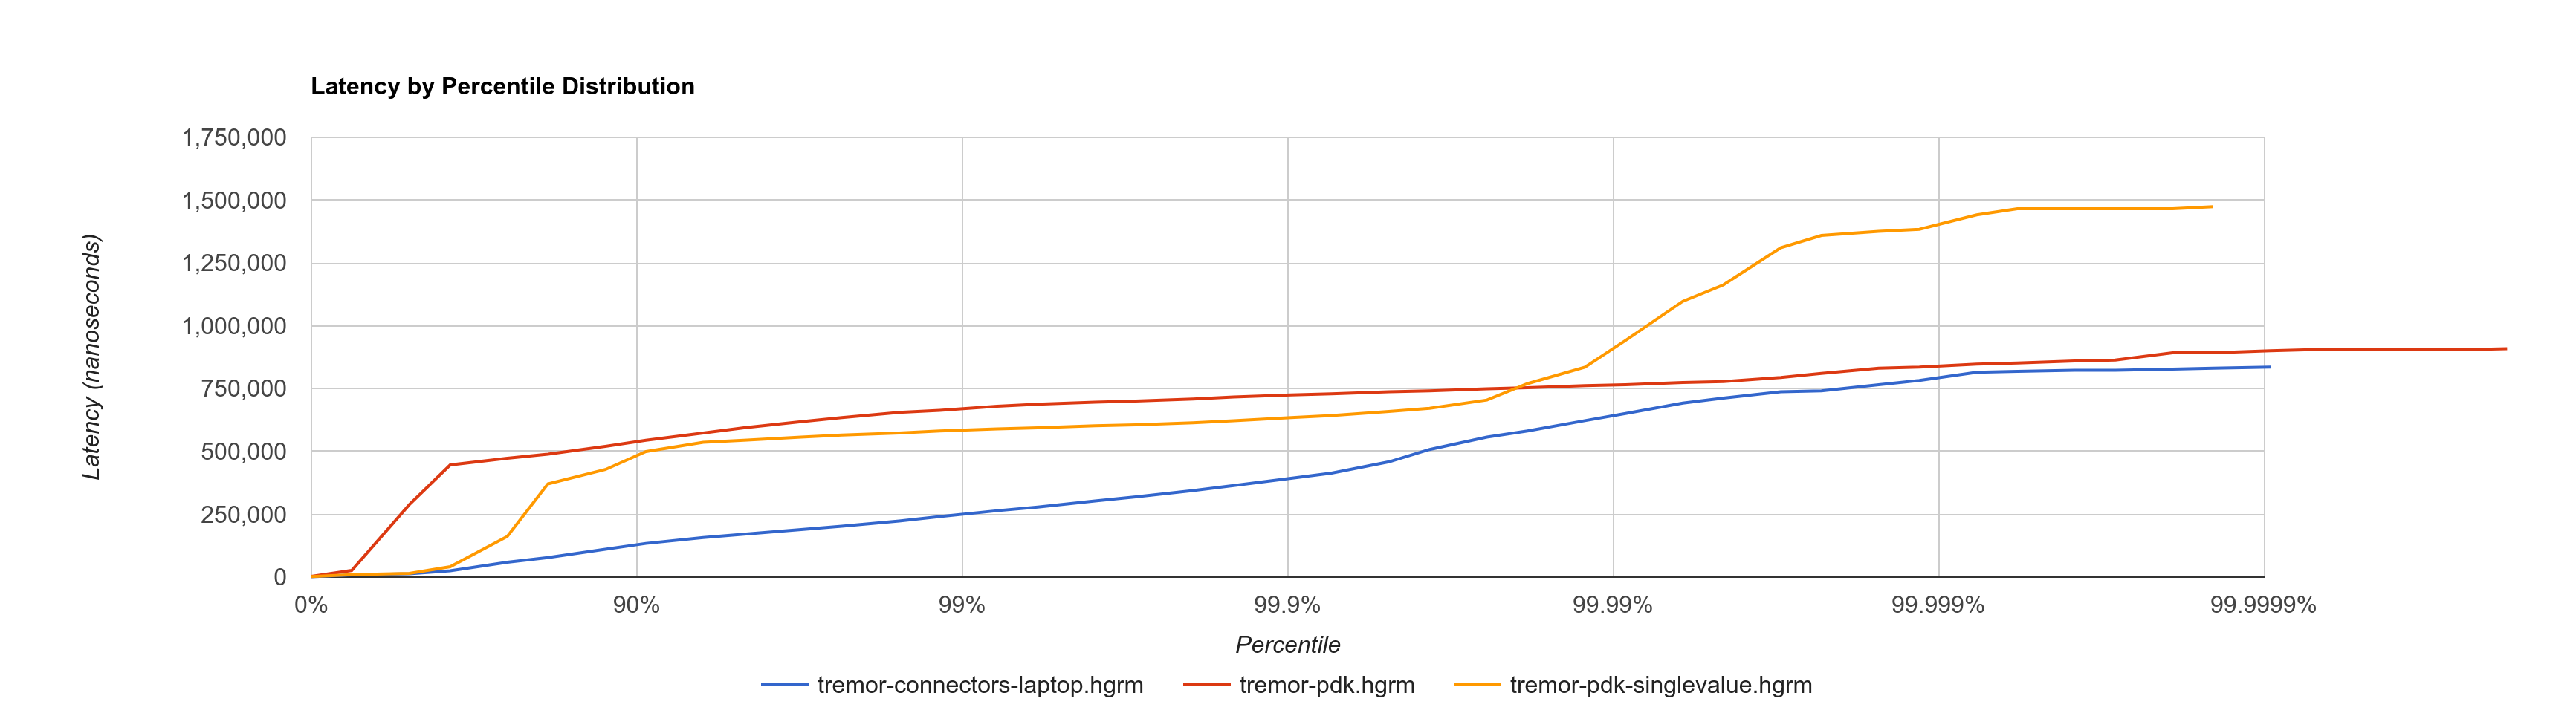
\includegraphics[width=\textwidth]{./Imagenes/histogram_pdk.png}
    \caption{Histograma con dos diferentes versiones del sistema de plugins,
    mejorando la latencia iterativamente. Concretamente, la mejora consiste en
    usar un único \code{Value}, en lugar de la copia \code{PdkValue} (ver
    Anexo~\ref{annex:abi}). La línea marcada como
    \code{tremor-connectors-laptop} es la rama original de Tremor.}%
    \label{fig:histogram_pdk}
\end{sidewaysfigure}

\begin{sidewaysfigure}
    \centering
    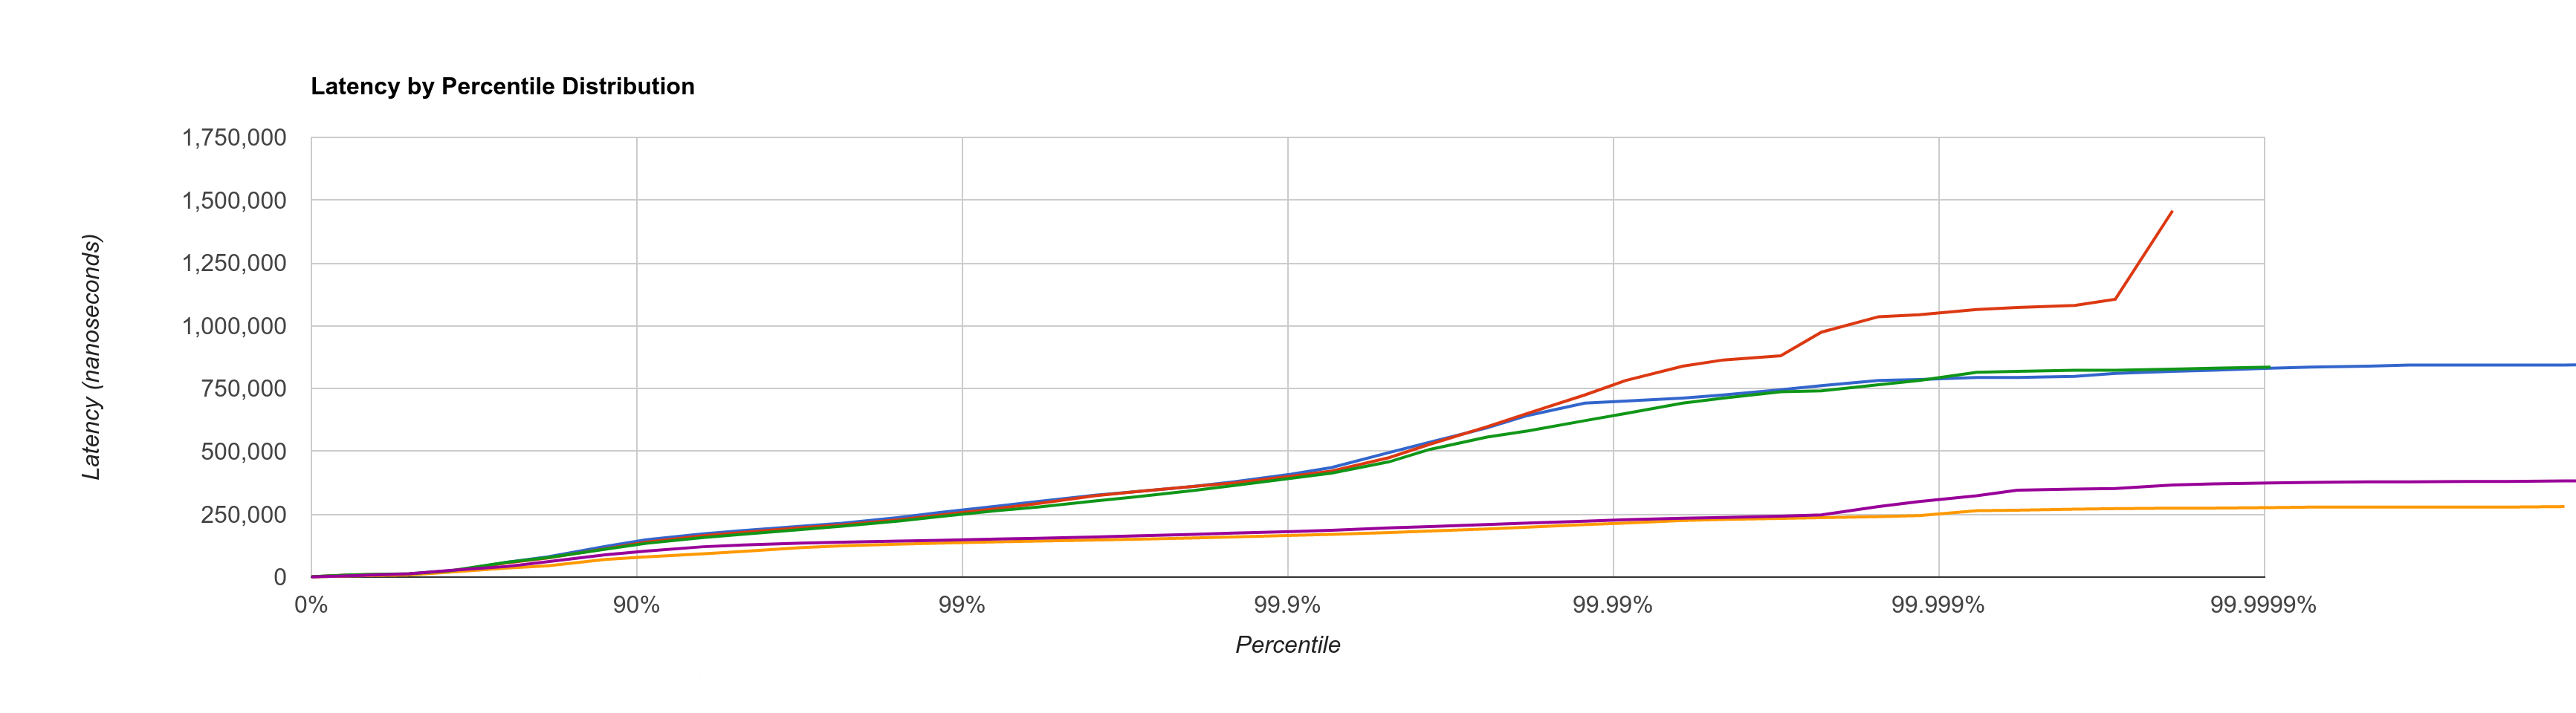
\includegraphics[width=\textwidth]{./Imagenes/histogram_variance.png}
    \caption{Las dos líneas inferiores son el mismo programa ejecutado en el
    servidor dedicado para medir su varianza. Las siguientes dos sobre estas es
    lo mismo con el portátil; la diferencia en varianza no es tan perceptible
    como se esperaba. Una mejora importante en la fiabilidad se consiguió
    realizando varias ejecuciones de calentamiento previas a las mediciones,
    como se puede ver en la diferencia de la línea superior, el portátil sin
    calentamiento, con las otras dos del portátil.}%
    \label{fig:histogram_variance}
\end{sidewaysfigure}

\begin{sidewaysfigure}
    \centering
    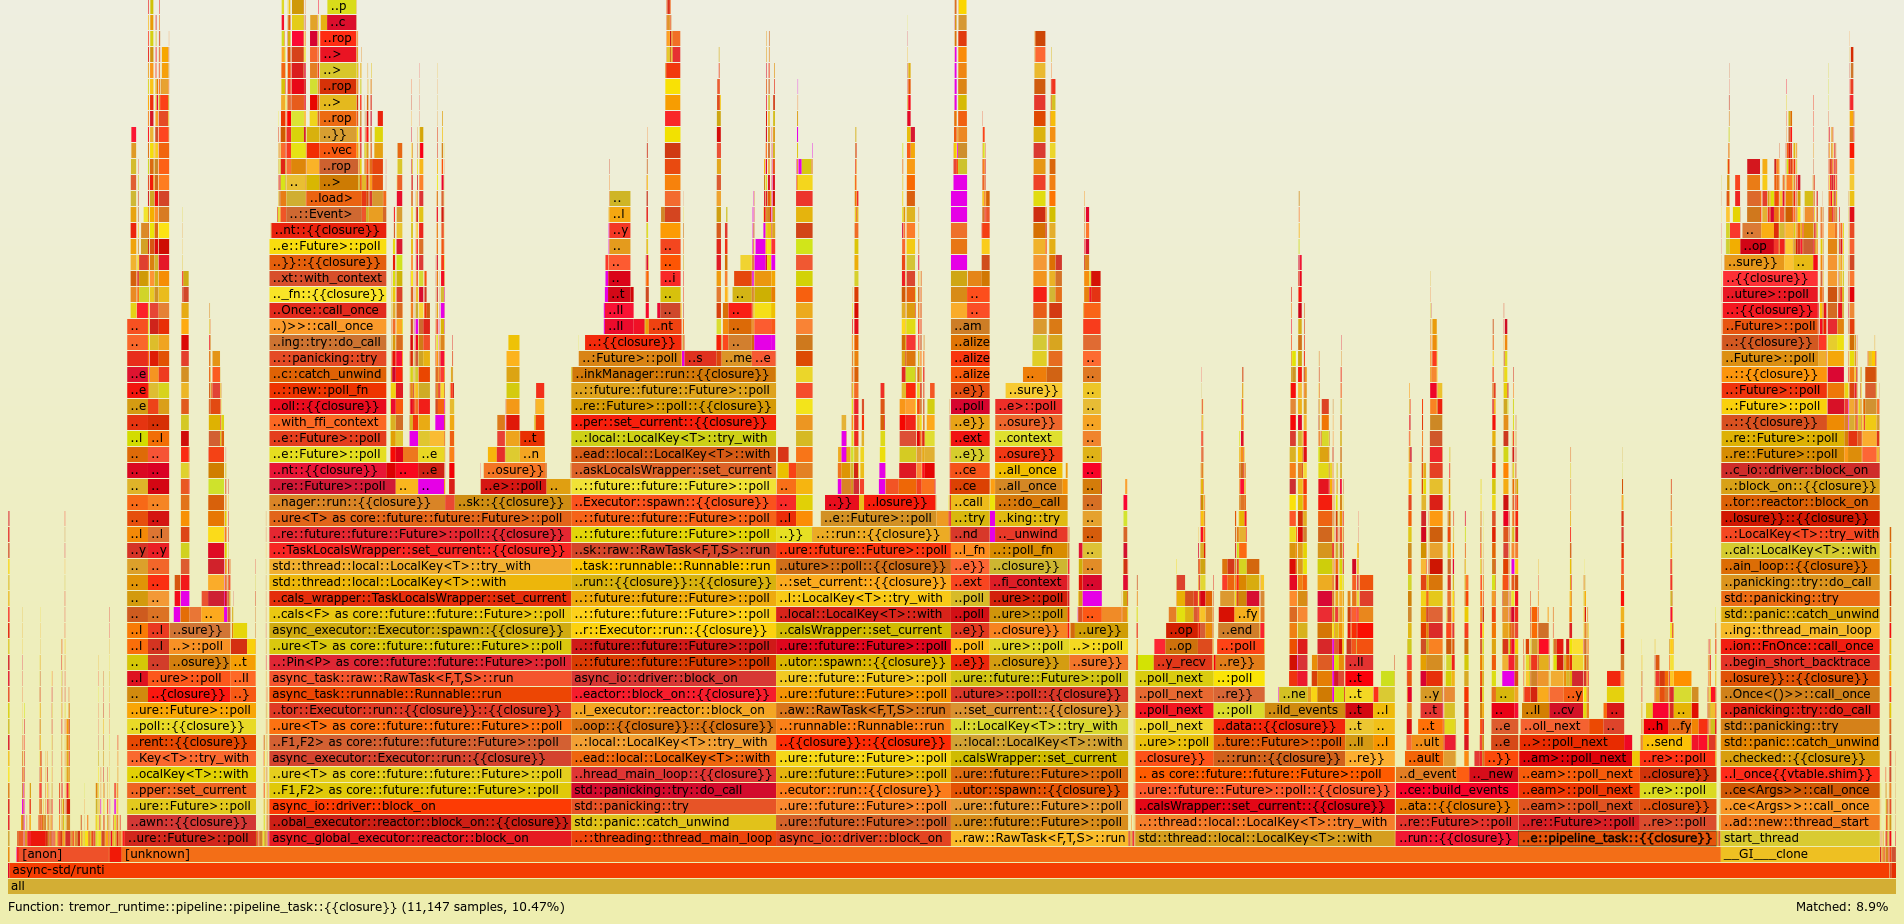
\includegraphics[width=\textwidth]{./Imagenes/without_value_conv.png}
    \caption{\emph{Flamegraph} con los porcentajes de ejecución de Tremor
    original, resaltando en rosa las conversiones de tipos realizadas.}%
    \label{fig:without_value_conv}
\end{sidewaysfigure}

\begin{sidewaysfigure}
    \centering
    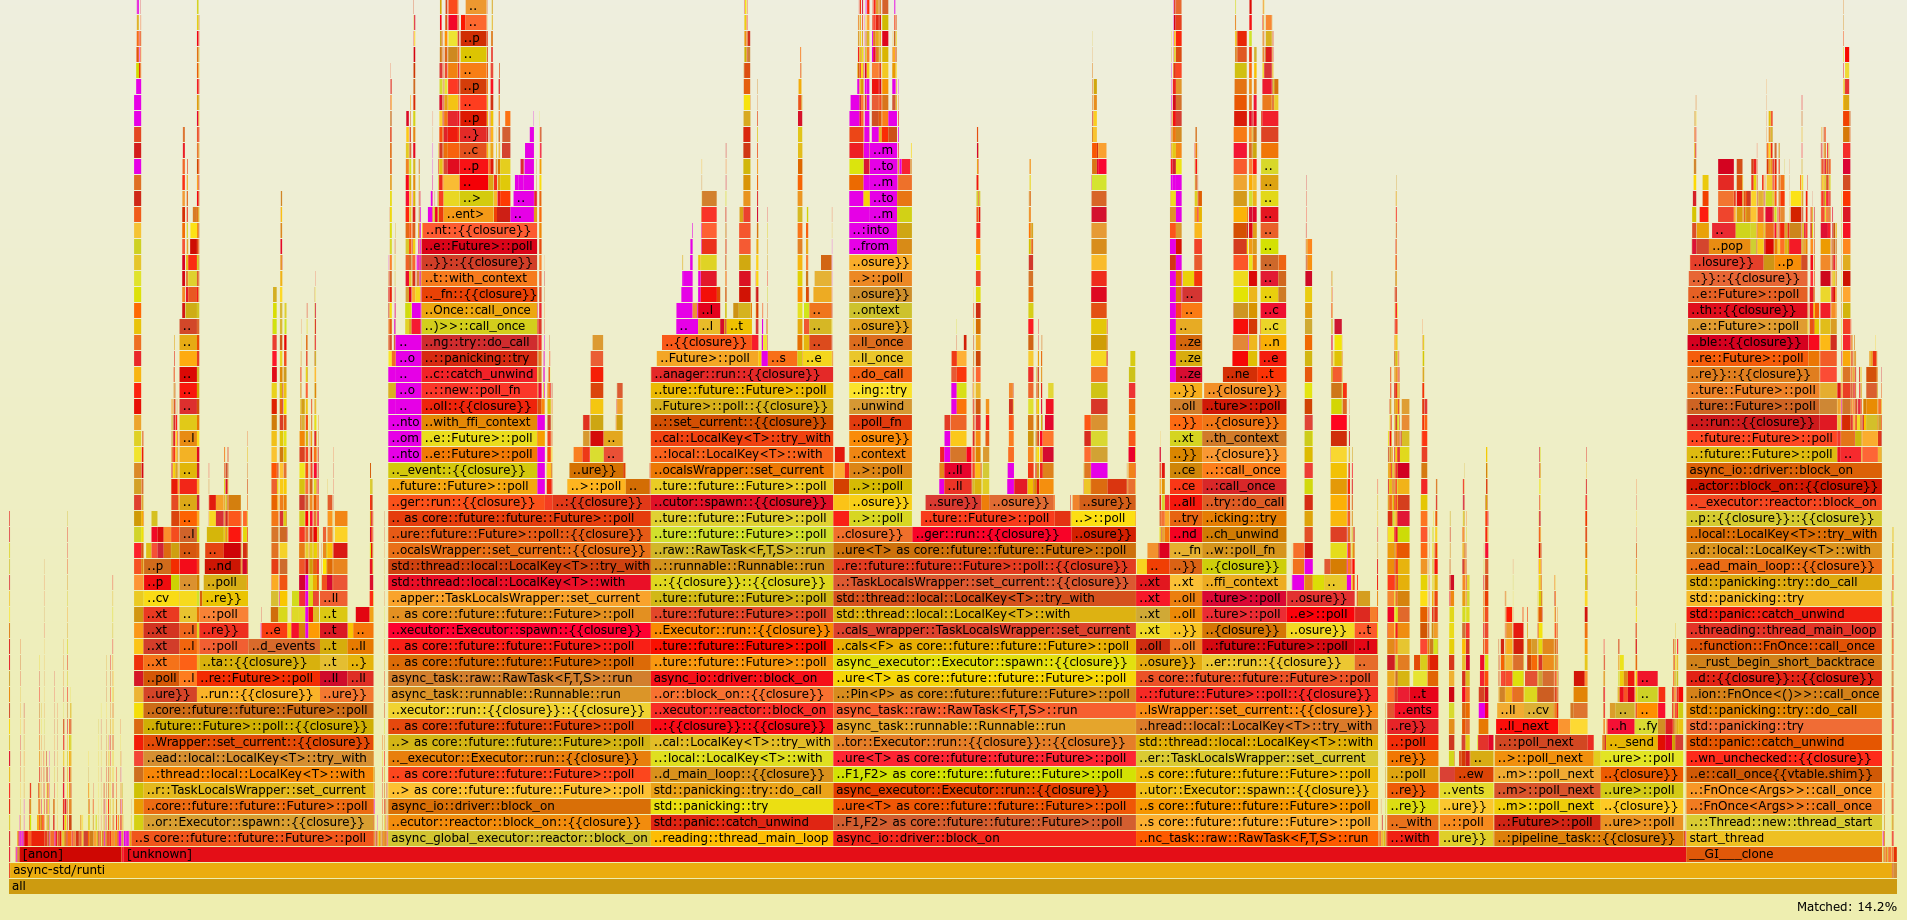
\includegraphics[width=\textwidth]{./Imagenes/with_value_conv.png}
    \caption{\emph{Flamegraph} una vez implementado el sistema de plugins. Las
    conversiones son más visibles ahora, puesto que es necesario para
    comunicarse entre runtime y plugins. Esta gráfica visualiza la degradación
    de rendimiento causada por conversiones de la librería estándar a \abistable
    y viceversa.}%
    \label{fig:with_value_conv}
\end{sidewaysfigure}

\begin{sidewaysfigure}
    \centering
    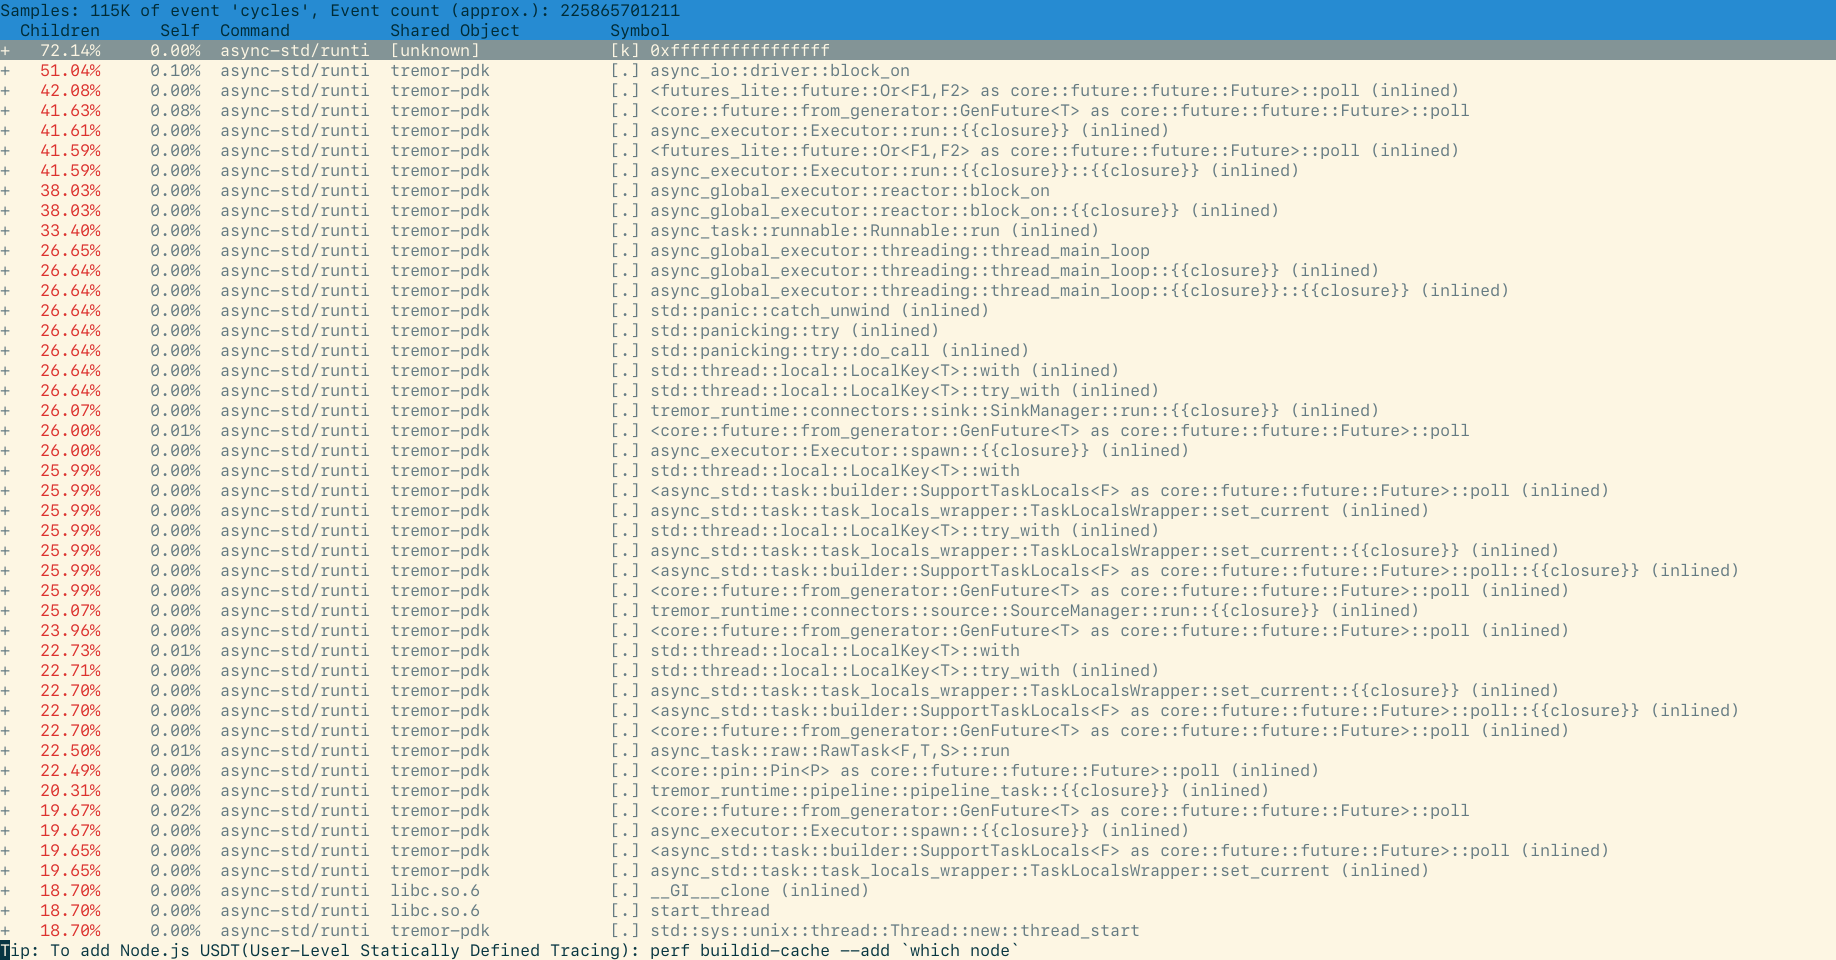
\includegraphics[width=\textwidth]{./Imagenes/perf_report.png}
    \caption{También se utilizó la herramienta \code{perf} para visualizar las
    secciones del programa más frecuentes en su ejecución. El comando completo
    es \code{perf report --no-children -i FILE}. El stack de programación
    asíncrona introduce gran cantidad de ruido, pero sigue pudiéndose distinguir
    por ejemplo \code{SinkManager::run} (ver Anexo~\ref{annex:tremor}), o el uso
    de \code{panic::catch_unwind} para pánicos seguros (ver
    Sección~\ref{sec:panics}).}%
    \label{fig:perf}
\end{sidewaysfigure}

\begin{figure}
    \centering
    \begin{minted}{bash}
#!/usr/bin/env bash

set -e

# Both paths must be absolute, and not use `~` or similars. Otherwise
# it won't work when ran as root.
TREMOR_DIR=/<fill-yours>/tremor-runtime
OUTPUT_DIR=/<fill-yours>/results
WARMUP_ROUNDS=0
BINARIES="tremor-connectors tremor-pdk"
BENCHMARKS="passthrough"

# Working with paths easily
get_dir() {
    dir="$TREMOR_DIR/tremor-cli/tests/bench/$1"
}
get_bin() {
    bin="../../../../target/release/$1"
}

# Validation step to avoid waiting for the benchmarks only for one of
# them to be incorrectly configured.
for bin in flamegraph; do
    if ! command -v "$bin" > /dev/null; then
        echo "ERROR: Binary $bin not available"
        exit 1
    fi
done
for name in $VALUES; do
    get_bin "$name"

    if ! [ -f "$bin" ] || ! [ -x "$bin" ]; then
        echo "ERROR: Binary $bin doesn't exist"
        exit 1
    fi
done
for name in $BENCHMARKS; do
    get_dir "$name"

    if ! [ -d "$dir" ]; then
        echo "ERROR: Benchmark $dir doesn't exist"
        exit 1
    fi
done
echo ">> Verification step passed"

# Setup
mkdir -p "$OUTPUT_DIR"
export TREMOR_PATH=../../../../tremor-script/lib:../../lib/
    \end{minted}
    \caption{Script usado para realizar las pruebas de rendimiento (parte 1/1).}%
    \label{fig:script_bench_1}
\end{figure}

\begin{figure}
    \centering
    \begin{minted}{bash}
# Finally running the benchmarks
for bench in $BENCHMARKS; do
    # Benchmarks only work if you're in the same directory, and then
    # always use relative paths.
    get_dir "$name"
    cd "$dir"

    # Warmup round, ran alternately for accuracy
    for i in $(seq $WARMUP_ROUNDS); do
        for name in $BINARIES; do
            get_bin "$name"

            echo ">> Warming up with $name ($i/$WARMUP_ROUNDS)"
            "$bin" test bench . > /dev/null
        done
    done

    for name in $BINARIES; do
        get_bin "$name"

        echo ">> Benchmarking $name"
        "$bin" test bench . > "$OUTPUT_DIR/${name}.hgrm"

        echo ">> Creating flamegraph for $name"
        flamegraph "$bin" test bench . \
            > "$OUTPUT_DIR/${name}-flamegraph.hgrm"
        mv flamegraph.svg "$OUTPUT_DIR/$name-flamegraph.svg"
        mv perf.data "$OUTPUT_DIR/$name-perf.data"
    done
done
    \end{minted}
    \caption{Script usado para realizar las pruebas de rendimiento (parte 2/2).}%
    \label{fig:script_bench_2}
\end{figure}
